\documentclass{article}

\usepackage{amsmath}
\usepackage{graphicx}
\usepackage[english]{babel}
\usepackage{hyperref}
\usepackage{xcolor}
\usepackage{float}

\usepackage[backend=bibtex, style=nature]{biblatex}
\addbibresource{refs.bib}

\title{DOE Proposal}
\author{Dinupa Nawarathne}
\date{September 2023}


\begin{document}

\maketitle

We can employ parametrized classifiers to perform a likelihood ratio test. Let's assume that $f(x, \theta)$ is a parametrized classifier trained to minimize binary cross-entropy (BCE) loss. Then the likelihood ratio for two parameters $\theta_{0}$ and $\theta_{1}$, is given by\cite{Rizvi:2023mws};

\begin{equation*}
	r(x| \theta_{0}, \theta_{1}) = \frac{p(x| \theta_{0})}{p(x| \theta_{1})} = \frac{f(x| \theta_{0}, \theta_{1})}{1 - f(x| \theta_{0}, \theta_{1})}
	\label{eq:Eq1}
\end{equation*}

In this study, we use a deep neural network (DNN) as the classifier. The DNN consists of five hidden linear layers, each containing 64 nodes. The ReLU function is used to activate the hidden layers, along with batch normalization layers. The final output is passed through a Sigmoid activation function. We use reconstructed information, denoted as $x = \{ \text{mass}, p_{T}, x_{p}, \phi, \cos\theta \}$, and particle-level information (generator level), denoted as $\theta = \{ \lambda, \mu, \nu \}$, as inputs to the classifier. The values of $\lambda$, $\mu$, and $\nu$ are uniformly sampled from the ranges $[1.5, 2.5]$, $[-0.5, 0.5]$, and $[-0.5, 0.5]$, respectively. The two classes used for classification are given in \autoref{tab:Table1}.

\begin{table}[H]
\begin{center}
\begin{tabular}{ |c|c|c| } 
 \hline
 $x$ values & $\theta$ values & label \\ 
 \hline
 mass, $p_{T}$, $x_{F}$, $\phi$, $\cos\theta$ generated with & & \\
 $\lambda = 1.$, $\mu = \nu = 0.$ & $\lambda = [1.5, 2.5]$, $\mu = \nu = [-0.5, 0.5]$ & 0 \\
\hline
mass, $p_{T}$, $x_{F}$, $\phi$, $\cos\theta$ generated with & &
\\ $\lambda = [1.5, 2.5]$, $\mu = \nu = [-0.5, 0.5]$ & $\lambda = [1.5, 2.5]$, $\mu = \nu = [-0.5, 0.5]$ & 1 \\ 
\hline
\end{tabular}
\caption{Physics variables with labels used in classification.}
\label{tab:Table1}
\end{center}
\end{table}


Note that the $\theta$ values are same in both classes. But the $x$ values are generated with different angular coefficients. Training the DNN classifier minimizing BCE loss with Adam optimizer\cite{kingma2014adam} will learn the likelihood ratio for any $\theta$ parameters. The loss curves are give in \autoref{fig:Figure1}

\begin{figure}[H]
\begin{center}
	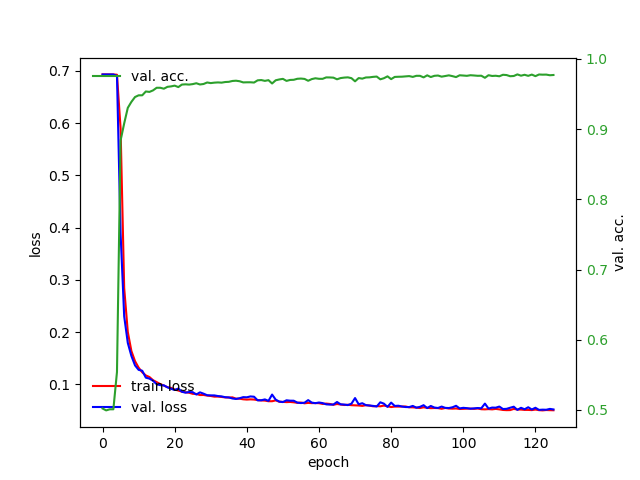
\includegraphics[width=8.0cm]{imgs/train_test_loss.png}
	\caption{\textcolor{red}{Training loss}, \textcolor{blue}{validation loss} and \textcolor{green}{validation accuracy} with epochs.}
	\label{fig:Figure1}
\end{center}
\end{figure}

After training the DNN classifier, we can perform a likelihood ratio test to extract unknown parameters. We can freeze all the weights and biases of the trained DNN classifier and change the parameters $\theta = \{\lambda, \mu, \nu\}$ by minimizing the BCE loss using the Adam optimizer. The two classes used in the fitting step are given in\autoref{tab:Table2}.

\begin{table}[H]
\begin{center}
\begin{tabular}{ |c|c| } 
 \hline
 $x$ values & label \\ 
 \hline
 mass, $p_{T}$, $x_{F}$, $\phi$, $\cos\theta$ generated with & \\
 $\lambda = 1.$, $\mu = \nu = 0.$ & 0 \\
\hline
mass, $p_{T}$, $x_{F}$, $\phi$, $\cos\theta$ with  &\\
unknown $\lambda$, $\mu$,  $\nu$ & 1 \\ 
\hline
\end{tabular}
\caption{Physics variables with labels used in classification.}
\label{tab:Table2}
\end{center}
\end{table}

The DNN classifier has a minimum loss at the optimal unknown parameter\cite{Andreassen:2019nnm}. As an example, the optimal value for $\mu$ exhibits a minimum loss at the injected value. This is shown in the \autoref{fig:Figure2}.

\begin{figure}[H]
\begin{center}
	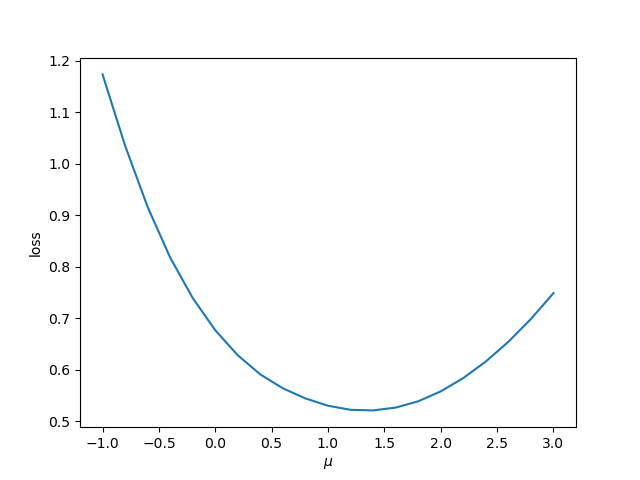
\includegraphics[width=8.0cm]{imgs/loss1D.png}
	\caption{Minimum loss at the optimal value.}
	\label{fig:Figure2}
\end{center}
\end{figure}

Using an gradient decent algorithm we can extract the unknown parameter efficiently. We use Adam optimizer to find the optimal value for unknown parameters. As shown in \autoref{fig:Figure3}, the fitted parameters converge to the injected values after some epochs.

\begin{figure}[H]
\begin{center}
	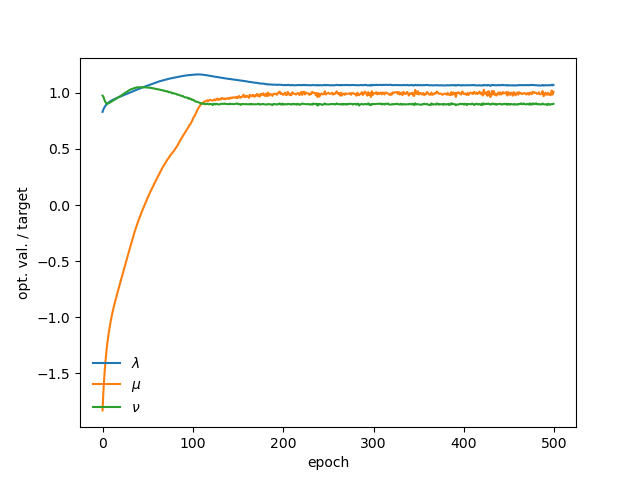
\includegraphics[width=8.0cm]{imgs/opt_fit.png}
	\caption{Fitted parameters converge to the injected value after some epochs.}
	\label{fig:Figure3}
\end{center}
\end{figure}

This method allow us to extract the Drell-Yan angular coefficients directly from the reconstructed detector information. Since we can use higher dimensional input features in training, we can use this method to incorporate full phase space when extracting the angular coefficients. This is an advantage compared to the traditional methods such as RooUnfold.\cite{Brenner:2019lmf}

An early result of this method was presented at the New Perspectives 2023\footnote{\url{https://indico.fnal.gov/event/59506/contributions/269963/}} and Neutrino Physics and Machine Learning 2023\footnote{\url{https://indico.slac.stanford.edu/event/8028/timetable/\#20230822.detailed}} conferences.

We are investigating how to incorporate generative models to improve the accuracy of this method\cite{Diefenbacher:2020rna}. We are using conditional variational autoencoders\cite{kingma2013auto} (VAEs) to generate new events with different angular coefficients. The idea is to classify VAE generated events with real events. Since likelihood of these two sets are very close, this method will help us improve the accuracy of the extracted parameters. A simple example of extracting the mean value of the Gaussian distribution is given in\autoref{fig:Figure4} and \autoref{fig:Figure5}.

\begin{figure}[H]
\begin{center}
	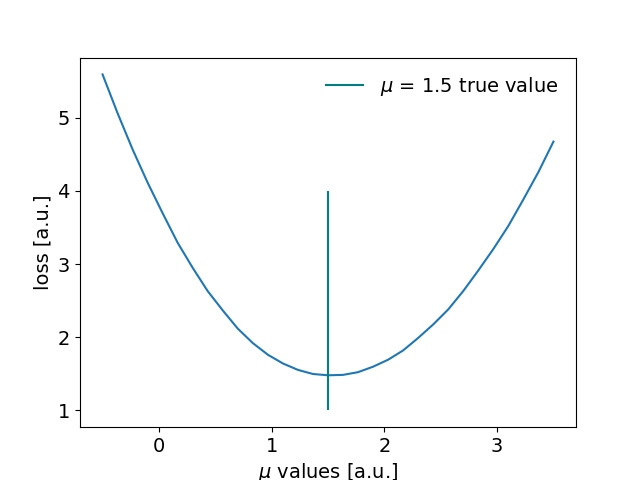
\includegraphics[width=8.0cm]{imgs/scan_opt.png}
	\caption{Loss has a minimum at the optimal value using VAE.}
	\label{fig:Figure4}
\end{center}
\end{figure}

\begin{figure}[H]
\begin{center}
	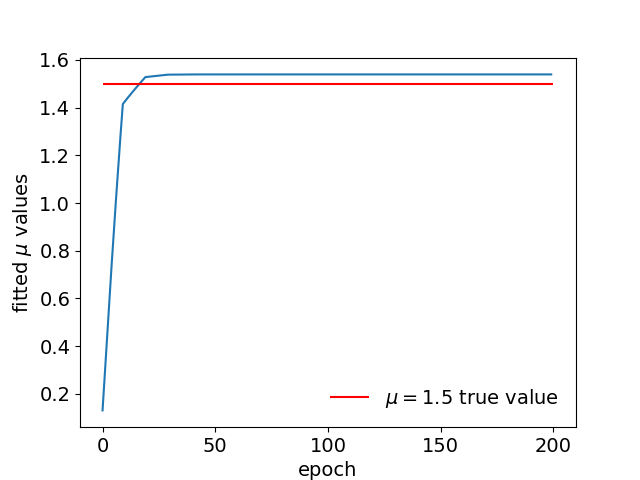
\includegraphics[width=8.0cm]{imgs/opt_params.png}
	\caption{Fitted parameters converge to the injected value after some epochs using VAE.}
	\label{fig:Figure5}
\end{center}
\end{figure}

The code for this study is in GitHub\footnote{\url{https://github.com/dinupa1/BMF/tree/main}} repository.

\medskip

\printbibliography
\end{document}